Results. Nice looking tables and charts of results.
\begin{figure}[ht!]
    \centering
    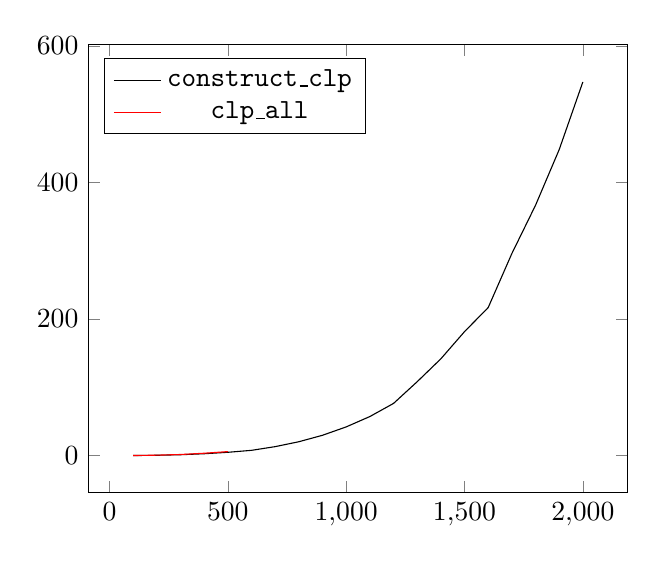
\begin{tikzpicture}
    \begin{axis}[
        legend pos=north west]

        \addplot[black] plot coordinates {
%            (0, 0.000012)
            (100, 0.120660)
            (200, 0.521410)
            (300, 1.307679)
            (400, 2.771161)
            (500, 4.879012)
            (600, 7.744716)
            (700, 13.167763)
            (800, 20.332959)
            (900, 29.800924)
            (1000, 42.052462)
            (1100, 57.228555)
            (1200, 76.425515)
            (1300, 108.207058)
            (1400, 141.722463)
            (1500, 181.548302)
            (1600, 216.743981)
            (1700, 295.849322)
            (1800, 366.523868)
            (1900, 448.033278)
            (2000, 547.087066)
        };

        \addplot[red] plot coordinates {
%            (0, 0.000001)
            (100, 0.155080)
            (200, 0.671939)
            (300, 1.656583)
            (400, 3.510805)
            (500, 5.887408)
        };

        \legend{\texttt{construct\_clp}, \texttt{clp\_all}}
    \end{axis}
\end{tikzpicture}

    \caption{Seconds used to solve all $s$ subinstances of randomly generated
             problems, when $b = 1$. The x-axis represents $n$, the number of
             edges in the network, i.e. the number of variables/columns in the
             QP problem. The y-axis represents the number of seconds used.}
    \label{fig:constructb1}
\end{figure}
